\begin{wrapfigure}[20]{r}{0pt}
		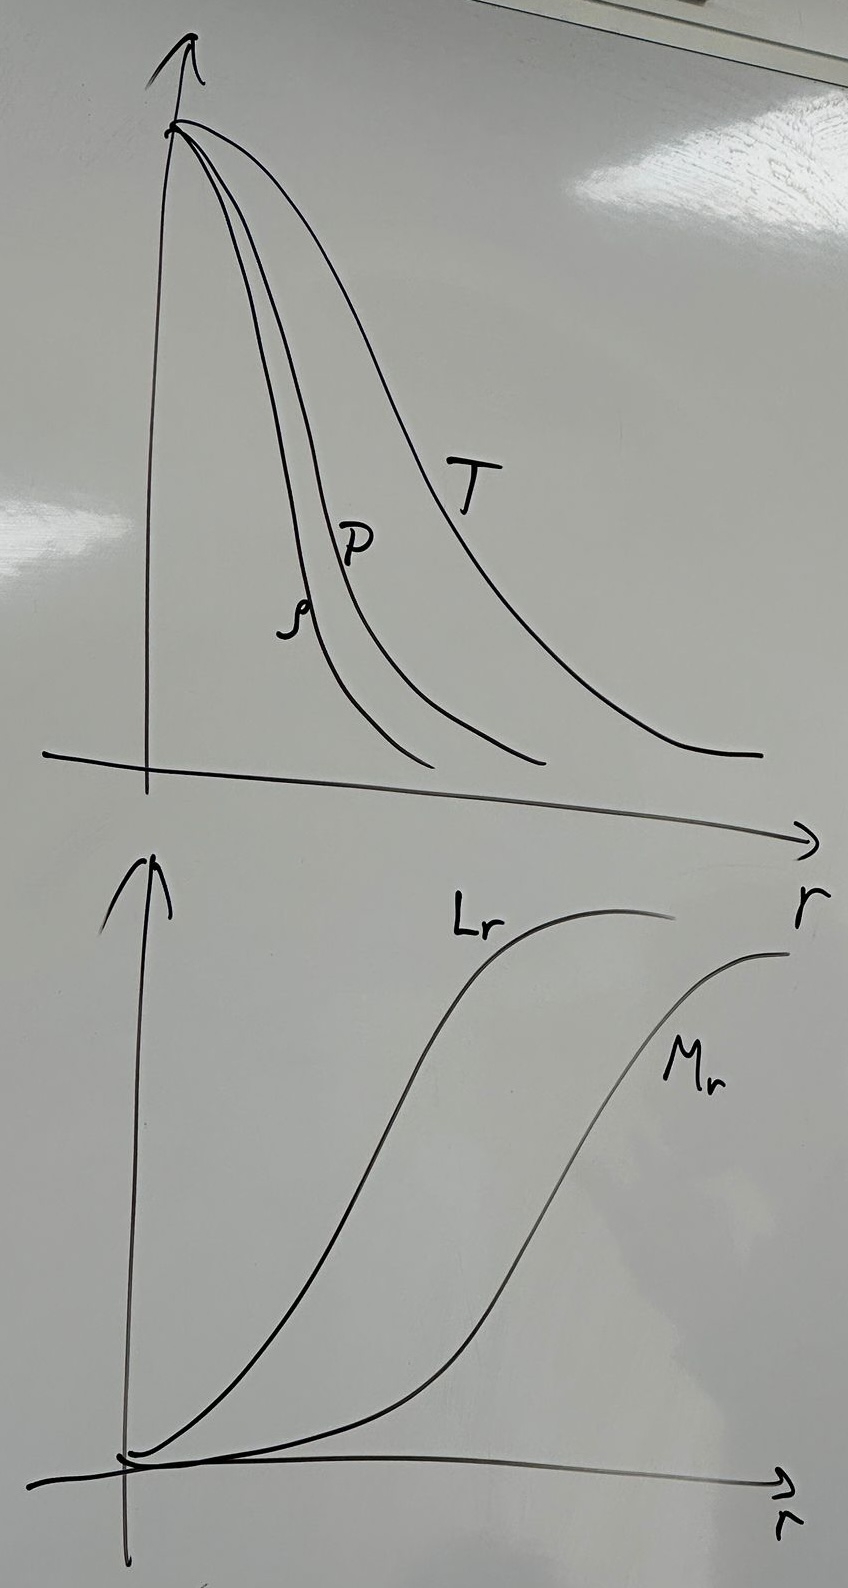
\includegraphics[width=0.3\textwidth]{images/WhatsApp-Image-2025-11-20-at-12.03.20.jpeg}
\end{wrapfigure}

For an approximate set of solutions we can assume that 

\begin{align}
	\left.T,P,\rho\right|_{r=R_*} = 0 && \left.M_r=L_r\right|_{r=0}=0 && \begin{cases}
		\left.M_r\right|_{R_*} = M\\
		\left.L_r\right|_{R_*} = L
	\end{cases}
\end{align}

In the process of diffusion, photons can undergo several kinds of interactions

\begin{description}
	\item [Bound-bound (Excitation)] $X+\nu \rightarrow X^*$.
	\item [Bound-free (Ionization)] $X^n+\nu \rightarrow X^{n+1}+e$. \\With $\sigma = \sigma_0\ins{\frac{h\nu}{E_0}}^{-3}$ for hydrogen and atoms with one electons.
	\item [Free-free absorption (Reverse bremsstrahlung)] 
	\item [Free-free e-scattering (Thomson)] which has a well known action cross section $\sigma_T = \frac{8}{3}\pi r_e^2$ where $r_e = \frac{e^2}{m_ec^2}$. Additionally, if there are ions in the area then if $\lambda \ll r_p$ there can happen Compton scattering and if $\lambda \gg r_p$there can happen Rayleigh scattering.
\end{description}

\begin{figure}[!htb]
	\centering
	\begin{subfigure}[h]{0.4\textwidth}
		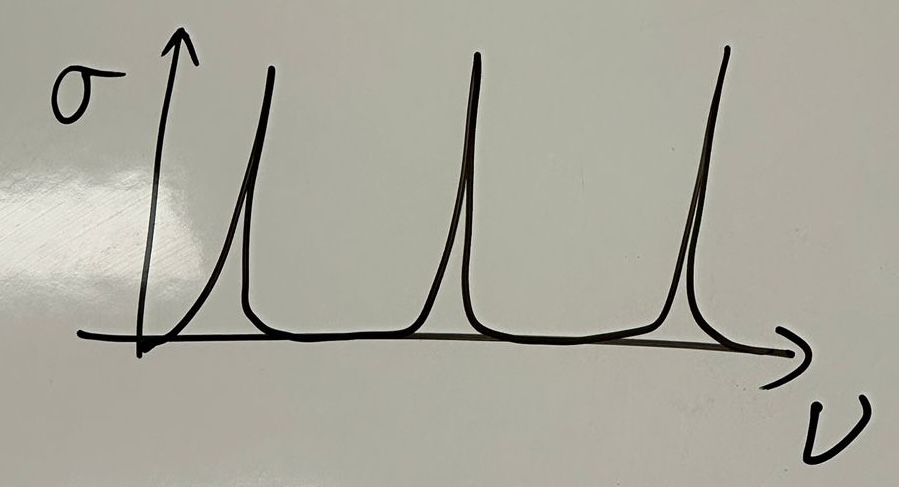
\includegraphics[width=\textwidth]{images/WhatsApp-Image-2025-11-20-at-12.03.21.jpeg}
		\caption{Bound-bound (excitation)}
	\end{subfigure}
	\begin{subfigure}[h]{0.4\textwidth}
		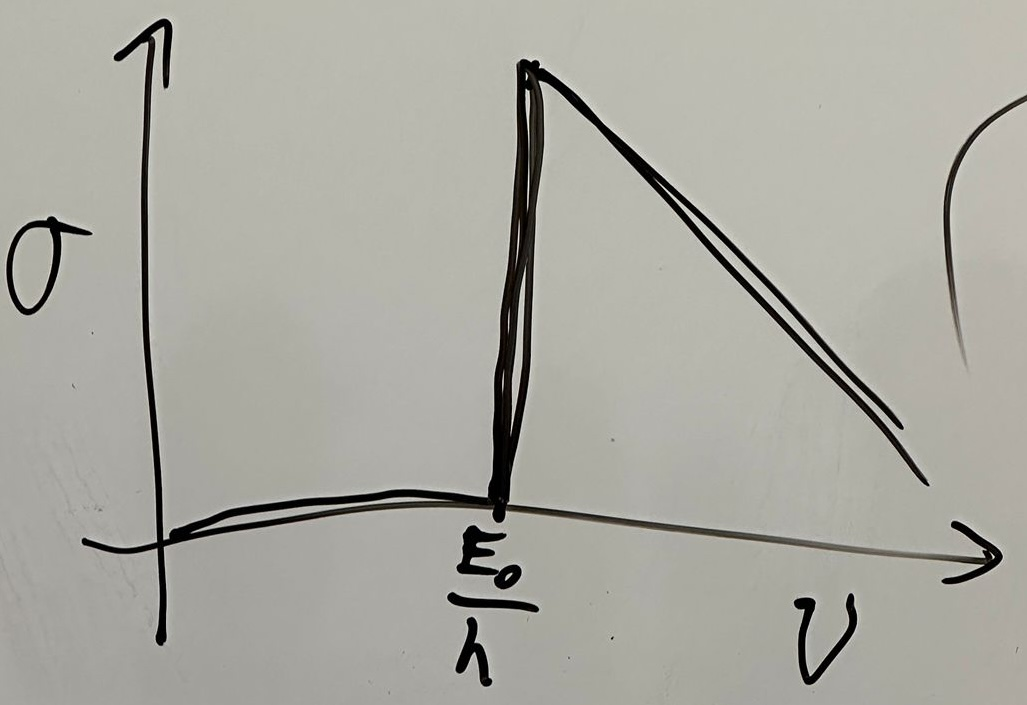
\includegraphics[width=\textwidth]{images/WhatsApp-Image-2025-11-20-at-12.03.21_1.jpeg}
		\caption{Bound-free (Ionization)}
	\end{subfigure}
\end{figure}